\section{Paper Sponsorships}
\label{sec:sponsors}
In addition to ads on our Digital Library, we will also be adding
advertisements to the papers themselves.
These advertisements will come in many forms, including standard banner
advertisements as well as increasingly popular native advertisements.

\subsection{Call for Advertisements}
Reach the largest holistic-minded audience in the entire northeastern United
States with an ad in the next ACM edition.\footnote{Wisdom disputes this claim, but we have the narrow computational tools to prove our publication and community have way more holism.}
Our readership is mostly devoid of energy vampires and is therefore suitable
for empath advertisers.
Where IEEE uses Western proof verification techniques, our broad-minded
audience validates mathematical claims in an intuitive holistic manner and will
bring that same spirit into evaluating the claims of your advertisements.
Our readers will engage with your brand through meditation and other
surprises.

\subsection{Banner ads}
Web surfers today have become accustomed to seeing banner ads on their favorite
websites.
Therefore, we will be incorporating these advertisements into all of our
papers.
Advertisements can be easily inserted into existing \LaTeX\ papers through the
use of the \texttt{\textbackslash figure} and \texttt{\textbackslash figure*}
constructs.
Of course, advertisements using the two-column \texttt{\textbackslash figure*}
construct will be considerably more expensive than their one-column brethren.
A standard single-column ad can be seen in \autoref{fig:law} while a
double-wide can be found in \autoref{fig:usa}.

\begin{figure}
\centering
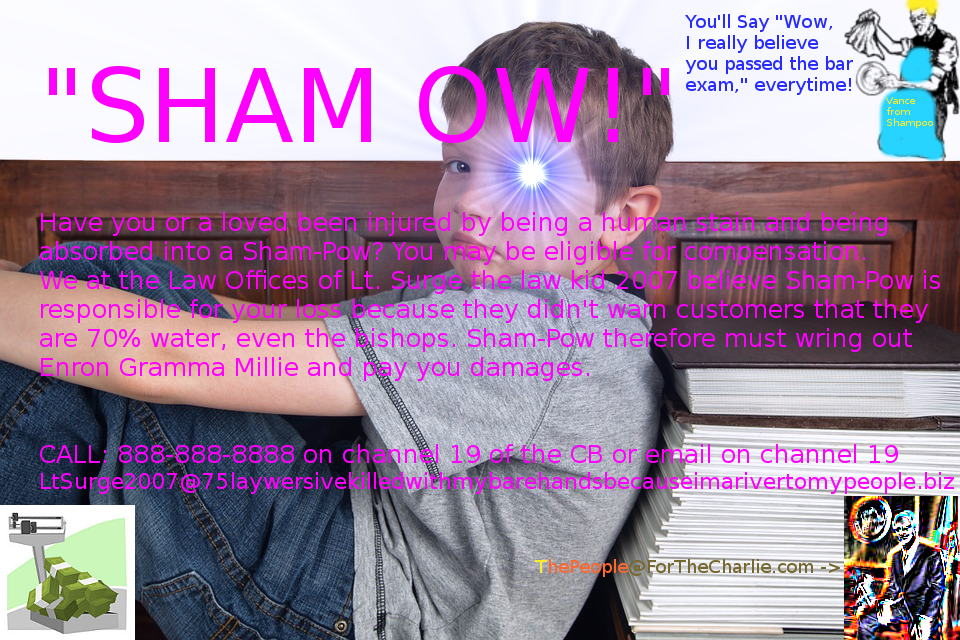
\includegraphics[width=0.45\textwidth]{figures/law-kid-ad.png}
\caption{Get your settlement today \cite{med-scale}!}
\label{fig:law}
\end{figure}

\begin{figure*}
\centering
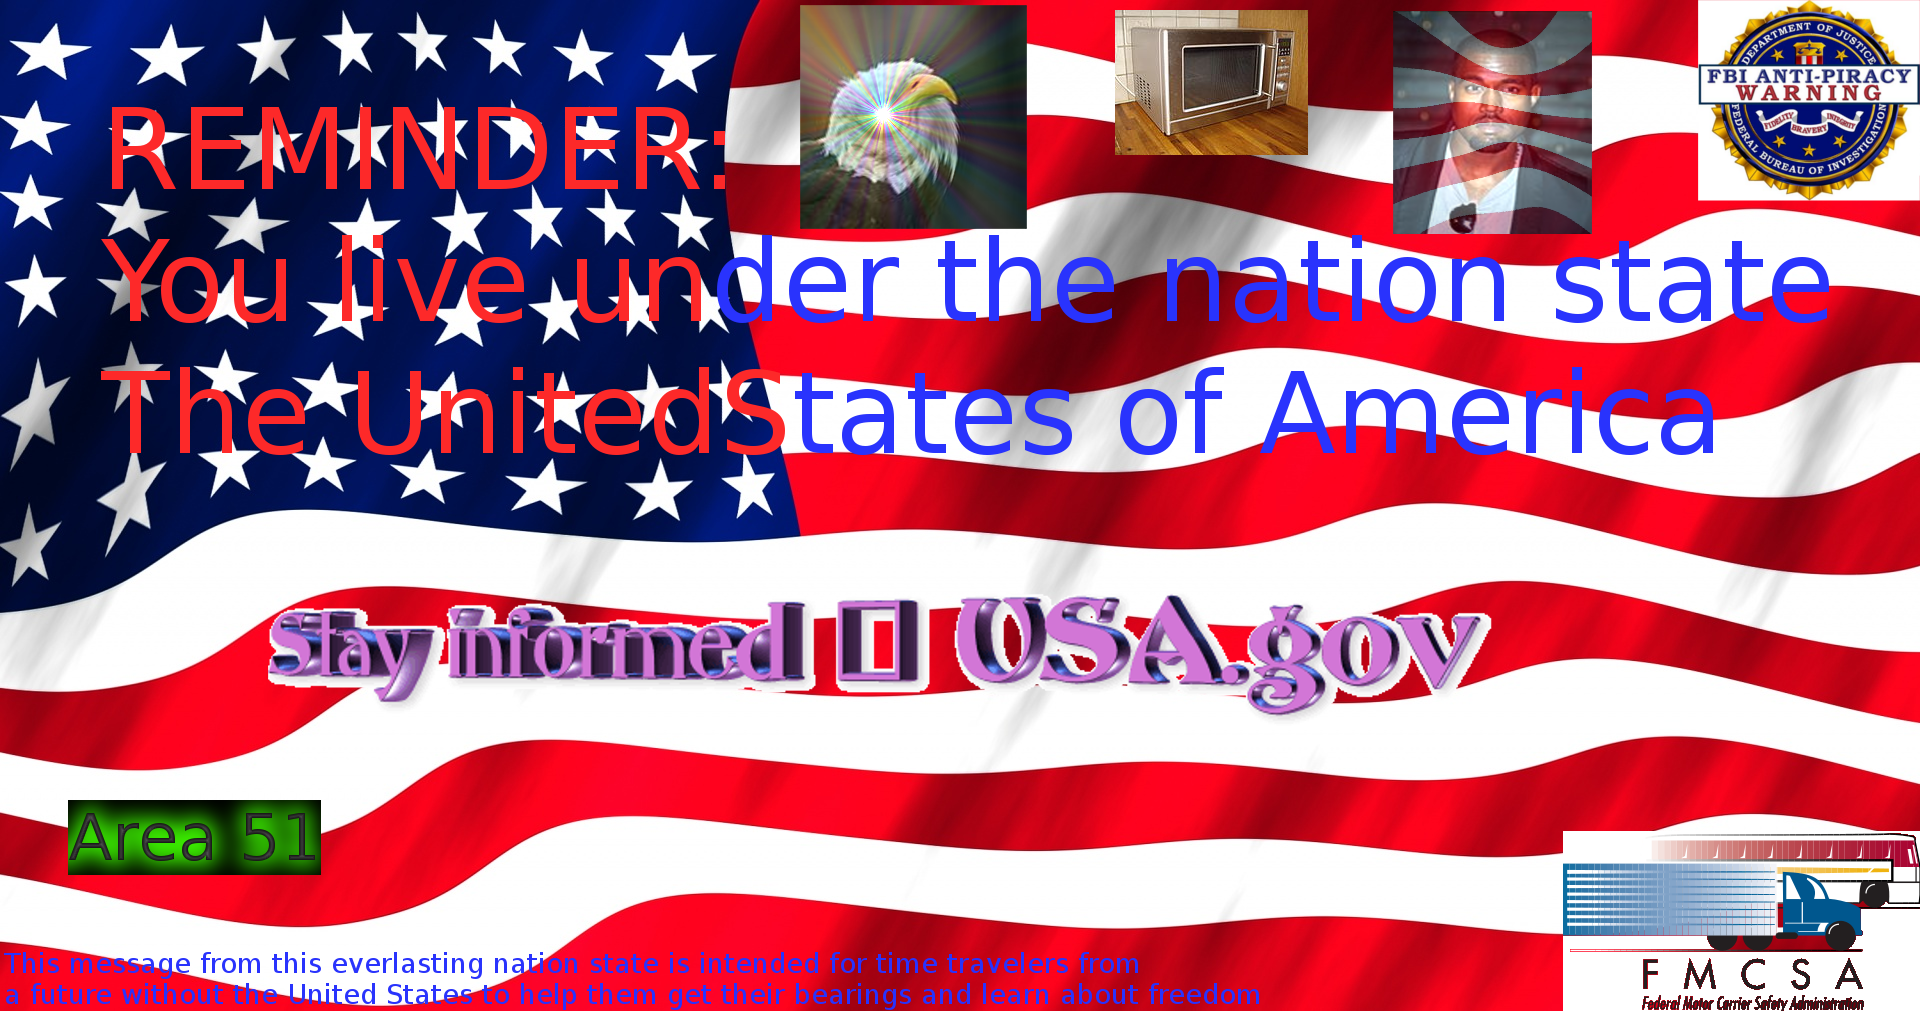
\includegraphics[width=0.95\textwidth]{figures/usa-ad.png}
\caption{We have near absolute power over you \cite{eagle, kanye, microwave}!}
\label{fig:usa}
\end{figure*}

For an additional fee we will also allow advertisers to embed autoplaying audio
into their paper ads.
While we aren't currently sure whether or not the PDF specification allows
this, we believe that there are sufficiently many ACM-loving PhDs at Adobe to
get this change  pushed into the spec.

\subsection{Ad-Enhanced Fonts}
Computer Modern is a staple of today's papers, but we believe that this font can
be monetized.
By replacing the characters in the default \LaTeX\ font with corporate logos
we can convey the same information in an ad enhanced way.
%The inspiring example of Claude Shannon proves it!



During each call for papers we will also put out a simultaneous call for
logos where companies can bid on desirable letters.
To avoid a Wingdings thing \cite{wingdings}, we require that the company
logo be a stylized version of the letter being replaced.


\subsection{Native Ads}
Native advertisements are advertisements meant to be disguised among the normal
content of a publication, much the way nutrition is disguised in the
kid-tested, parent-approved, and flavor packed Flavor Paks.
They are written in the same style as the publication and appear alongside
unsponsored content in an attempt to make the reader believe that they are
reading the original publication and not an advertisement \cite{native}.

At paper registration time, authors will be given ad copy\footnote{Beware that
  accessing our site over Tor or other anonymizing networks can result in ad
copy presented in another language.}
  to integrate into their work.
Each paper is required to have at least one section advertising the product
that was assigned to the research project.
As these ads must be indistinguishable from the rest of the paper, an
advertisement that is recognizable as an ad will result in the rejection of the
paper.
The ad section must be at least one page long, but there is no upper bound on
native ad length.
We recognize that this will eat into the page limits of some conferences so we
will allow authors to deduct the length of the native ad from their total paper
length provided that the length of the native section alone exceeds the total
page limit.
Authors can claim this deduction by filing a Form 8843 with their paper
submission.

\subsection{Branded mathematical objects}
\label{sec:brands}
We believe there has been a missed opportunity in the field of mathematics to
increase brand awareness.
Therefore, we propose branding mathematical objects by associating every single
set with an individual brand.
Brands can purchase large collections of sets at a discount.
While most sets are cheap, some more famous sets will be priced higher to
reflect their higher market value, similar to domain names.

Authors referencing any given set must reference the brand of the set any time
the set is referenced, regardless of the format the set is presented  in.
Additionally, royalties must be paid to the owner of the set.

We are excited to announce that our first partner in this endeavor will be
Chili's Grill $\|$ Bar,\footnote{The chill of severity and emptiness in every
bite.} which has purchased the rights to the set of natural
numbers.
From here on, authors must refer to this set as the Chill's Grill $\|$ Bar Set of
Natural Numbers \(\mathbb{N}\).

\subsection{Investor Science Dispute Settlement}
We have founded an Investor Science Dispute Settlement (ISDS) court to protect
businesses from results that may damage their reputation or profits.
If a research project is found to be damaging, the authors must either retract
the paper or pay a settlement equal to the estimated losses suffered by the
company, or 25 US Dollars\footnote{In the present, United
  States Dollars are the one true world currency.  The value of \$25
in yesterday's Austro-Hungarian forint is not known.}, whichever is greater.
For example, if some agitator finds that the complexity class PLS is in PPP
relative to some oracle, they will dash the hopes of the typical Sparrow Soap
consumer, leading to hygiene neglect\footnote{At least influenza feels like
something.}
Therefore, Sparrow Soap may use the IADS court to mitigate their losses from
this finding.
Moreover, since Sparrow Soap owns both of these complexity classes as defined
in section \autoref{sec:brands} their assets will lose value and
this loss must be compensated by the offending authors.

Several ``bloggers" and fuddy-duddies fixated on a staid notion of ``truth" (lacking the agility and dynamism that characterize a proactive, change-driven science) have deigned to argue that this arrangement gives particular corporations undue influence over science and could lead to corruption. These agitators are, of course, anti-science zealots who fail to realize the emancipatory potential of this settlement system. Much as the visionary rulings of Anthony Kennedy and others have opened up our politics to make it more responsive to democratic speech, ISDS will make science more responsive to the needs of democratic actors, like 501(c)(4) ``social welfare" nonprofits. Welfare! It will democratize our understanding of reality, taking science out of the smooth, mildly scented ivory tower and cramming it into the ad-plastered public square. Science is agoraphobic but its future is in the agora of the brainscape---the marketplace of ideas---so (to coin a term) ISDS is the deagoraphobification of science. Science cannot ignore society. Science must come to where the flavor is.

What of the science that does get published? The agents who do get economically controversial results published are likely to be powerful entities in a society with concentrated private economic power, some argue.
On the contrary, we contend that such restrictions on publication enable the
purest form of democracy, the ``mischief of factions."
Simply put, ISDS provides a powerful mechanism of checks and balances. If Hot
Packets wants to get their signature snack food placed on the government's food
pyramid, it would need peer-reviewed science attesting to its beneficial health
effects (such as an appearance on the Doctor Conflict-of-Interest show, where
the titular doctor attests to its miracle superfood status, or a research
paper). To appear in print, it would have to pay off claims from competing
superfoods such as Berry Loops or Jazz Flakes.
But, say, if the parent companies of all products for sale wish to merge,
research touting the consumer benefits of concentration would have little
trouble passing ISDS review.
 Approved ideas get approved quickly, and the system works!

ISDS also applies to scientists in their personal lives. If a scientist, for instance, posts to social media video of an alleged bad encounter with an internet service provider's customer service representative or video of hose water burning---and ISDS tribunal statisticians (employees of the ISDS corporate community, on rotation) determine that, as a result of these actions, shareholders lost value---then the economic terrorists promulgating this ticker-tanking tripe will have to compensate all shareholders for the drop in share price, as well as the social media platform monopoly's shareholders (if applicable; scientists should not be using free, distributed social networks but may use privately held proprietary platforms) for the shame they've brought to the platform even if share price was unaffected. This way, the integrity of the scientific process is protected---and scientists represent science with honor---in all spheres, not just peer-reviewed journals.   

\subsection{ACM Classifieds}
For additional funding we allow individuals to take out classified ads in the
following sections.
To keep costs low, the ACM does not vet any classified postings.

\paragraph{Dropped Packets}
Dropped Packets serves as the traditional missed connections section of the
classifieds.
While this could be used to contact that cutie from the latest conference, we
believe that it could also be used to publicly shame those who miss meetings.
Some examples include:

\begin{enumerate}
  \item Missed Connection: Lost Tofutti Cutie at last conference, fell behind the freezer before I could read it. No reward. I just want a witness to my experience.

  \item Damn it Deborah, you were supposed to bring bagels to the DARPA
Tactical Anti-\censor{blank} HAVE BAGEL Infiltration \censor{long blank}
(DTA\censor{b}HBI\censor{bb}) meeting!

  \item I was hiding in your closet at 1 Infinite Loop Apt. \# 2 and you were home and you took a shower but you grabbed wrinkled clothes from your laundry hamper and didn't access your closet, and I hadn't eaten anything but moths for many hours, so I slipped out of your home but just know you are loved.
\end{enumerate}

\paragraph{Job Queue}
The Job Queue section contains odd jobs for trained Computer Scientists looking
for instant internet income.
Those who pay extra will get a free AirDancer\footnote{Placed at the discretion
of the ACM in the ACM AirDancer Oasis in the Black Rock Desert in Nevada in
solidarity with the aliens illegally detained in Area 51. The AirDancers may
be used by the aliens to communicate with their home world about the status of the part needed to keep the AirDance of the cosmos going.}!




\paragraph{Overclock}
Overclock is a section for performance enhancing drugs tailored for computer
scientists.
This section is mostly targeted at the Hacker News \cite{hn} crowd who exclaims
the benefits of small amounts of LSD for enhancing productivity at work
\cite{microdose, lsd-song}.
Although we can't promote the use of illegal drugs our editor is so strung out
on ``road cheese" that she won't notice.
% http://www.forbes.com/sites/robertglatter/2015/11/27/lsd-microdosing-the-new-job-enhancer-in-silicon-valley-and-beyond/#323d0dab114d

\subsection{Check Scams}
\iffalse
Digital is the new normal. Digital is the new ubiquity. Digital is the new cuddling. Digital is the new word we use to paper over our alienation with the capitalist mode of production at a time when socialism is possible.

We are now living in a world of 0s and 1s---or, if you prefer, sharks and minnows. The transformative power of this new digital world has been fully realized. Nothing can get more digital. It's either digital or it's not. And by now everything that's ever going to be digital has already become digital. We must accept this fact of this hardscrabble, accept-or-be-accepted world.

With our new digital world comes new digital innovations. Every brand, every person, and every personal brand is now a digital native. Digital is native and native, digital. Every transistor will be able to heal itself without consulting a physical medicine man. Big data, hot data, slow data, medium data, dirty data, long data, cold data, transient data, live data, cubed data, and target-rich data. But data is just a story, a narrative, and though every brand tells an authentic story, a brand is more than a story. The universe is not a story.

Thus, we will need to move beyond digital because digital is just story-telling. What matters is physical. Action potentials sparked by sensory inputs---sight, taste, ESP---and other action potentials. Statues of Jesus being carried by helicopter. Nothing is more authentic for consumers than the physical, than an action potential. In a world where everything is phony, only an action potential---even one involved in the process of telling a brand's story---is real.

Digital embodies the lifestyle and personality of the ACM author. But the ACM author exists in a physical space. Prior to the open-adcess revolution, the ACM author had to transact in this physical space to release a paper (digital locker room talk) in an ACM journal (digital locker). The revolutionary open-adcess model is America-first, digital-second. Now authors need never leave their digital hidey-holes by transferring funds to the ACM and, through fractional-reserve banking, creating physical changes in the non-digital sectors of our digital economy. 

But an author need not remain ensconced in the stately pleasure-dome of digital. In fact, when an author chooses to transact in the physical space, the open-adcess model empowers the author to not only avoid paying the publishing fee but also to get on the road to getting paid for their articles because authors deserve more.
\fi
Recent accounting innovations surveyed in two review articles and one major
motion picture \cite{ftc, check-scams, mich} enable the ACM to write large
checks to authors. In return, authors simply have to write a small check to
cover transaction fees before the large check clears.

\begin{figure}
\centering

\includegraphics[width=0.45\textwidth]{figures/ad.jpg}
\caption{Have you seen this boy? He's a great catch! He's not very bright, and he has your brother's thighs, those Goodman thighs. He's no Clark Gable, but he's \checkmark tall \checkmark detoxing from that juice craze, oh such a thrill \checkmark the doctors say he has sensory interests others find unusual \checkmark probably better with these checklists than I am \checkmark almost certainly willing to testify as an alibi, no questions asked. That's a rare attribute these days. That boy, I worry, though, I worry. He doesn't eat. But he's got no one, it kills me. You know, both of the Ableman kids, they had the Internet make the shidduch. I hope if I send this to these computer science people it gets on the line.}
\end{figure}

\begin{figure}
\centering
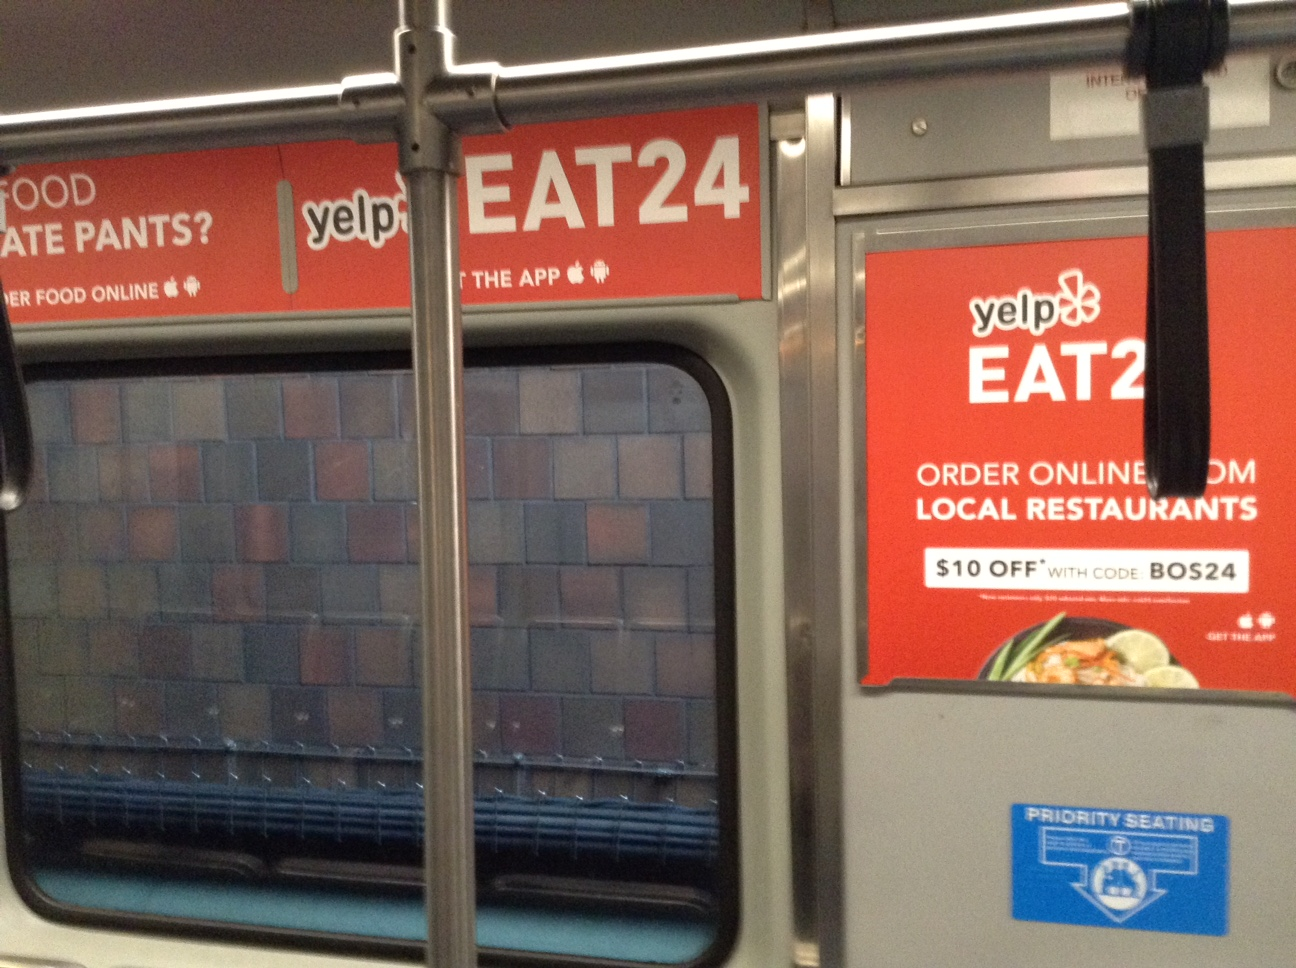
\includegraphics[width=0.45\textwidth]{figures/cambridge.jpg}
\caption{Visit beautiful Cambridge, MA. ``Where class privilege goes to reproduce itself.''}
\end{figure}

\begin{figure}
\centering
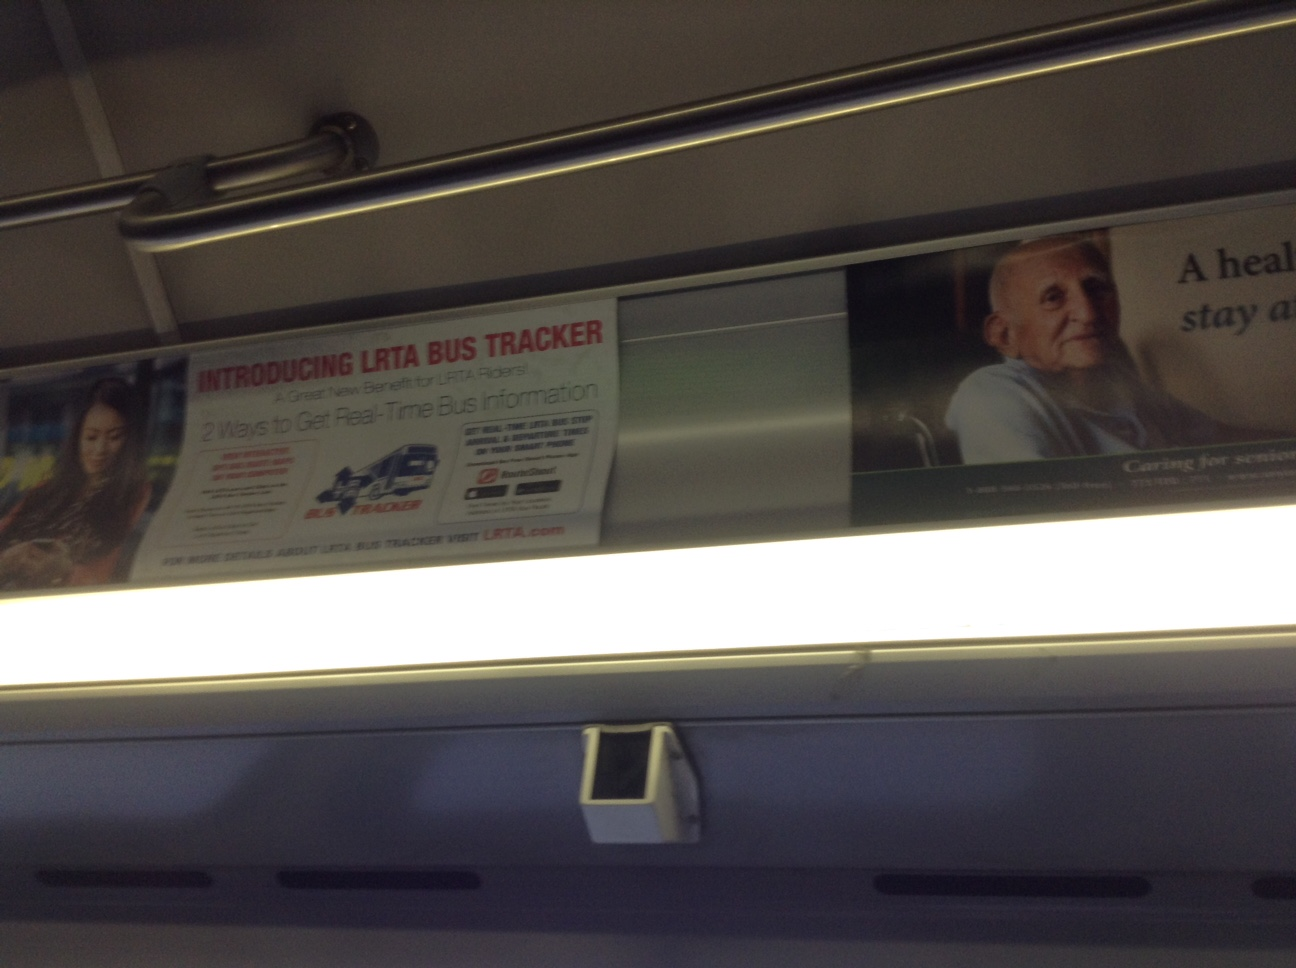
\includegraphics[width=0.45\textwidth]{figures/lowell.jpg}
\caption{Visit Lowell, MA. ``Where}
\end{figure}

